\chapter{Introduction}
\label{ch:introduction}

This Bachelor thesis is done by Simon Barras and supervised by Frederic Bapst
and Jean Hennebert.
The customer Paolo Calafiura is a physicist and computer scientist at the \acrfull{lbl}.
To do this project, I am moving to Berkeley, California, for ten weeks.
The goal is to explore a way to improve the performance of the project Celeritas,
which is a particle physics simulation software accelerated by \acrshort{gpu}s.

The two main customers are \acrshort{cms} and \acrshort{atlas}, two experiments
are made at the \acrfull{cern} with the \acrfull{lhc} and run
their simulation with Geant4.
They are both using Geant4 and they have not committed to using Celeritas
beyond an initial evaluation.
Detector simulation is used to validate and calibrate the algorithms used to
estimate the properties of the primary particles from the observed detector data.
The main goal of the thesis will be to optimize a GPU-accelerated version of
the Prince Dormand algorithm~\cite{princeDormand}, a
Runge-Kutta solver~\cite{Runge-Kutta-methods} for the differential equations
governing the trajectory of particles in a non-uniform magnetic field.
This work will improve the project Celeritas~\cite{Celeritas-Project} which may
replace Geant4~\cite{geant4} in the future.

The \acrshort{atlas} experiment tracks the path of particles in the detector and
produces coordinates points where particles traverse the sensors.
Figure \ref{fig:introduction:particles:tracking} represents this experiment.
\begin{figure}[ht]
    \centering
    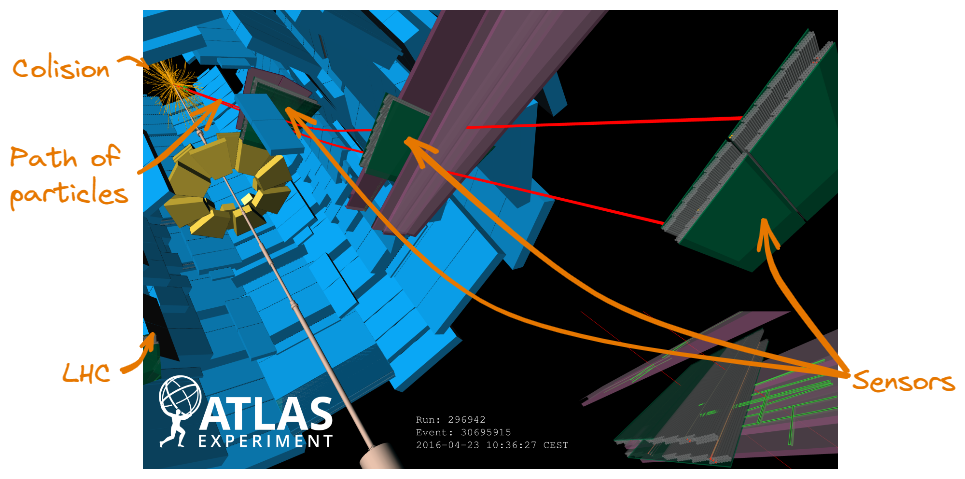
\includegraphics[width=0.85\textwidth]{05-resources/img/spec/experiment-atlas.excalidraw.png}
    \caption{ATLAS experiment at CERN~\cite{atlas-experiment}}
    \label{fig:introduction:particles:tracking}
\end{figure}

\section{Lawrence Berkeley National Laboratory}
\label{ch:introduction:lbl}

The \acrfull{lbl} is a national laboratory in Berkeley, California.
It is managed and operated by the University of California for the \acrfull{doe}.
The lab is situated in the hills of Berkeley and it is composed of many buildings
and has a beautiful view of the San Francisco Bay (see Fig.\ref{fig:introduction:lbl:view}).
This laboratory is mentioned in the recently released movie by Christopher Nolan,
"Oppenheimer".

\begin{figure}[ht]
    \centering
    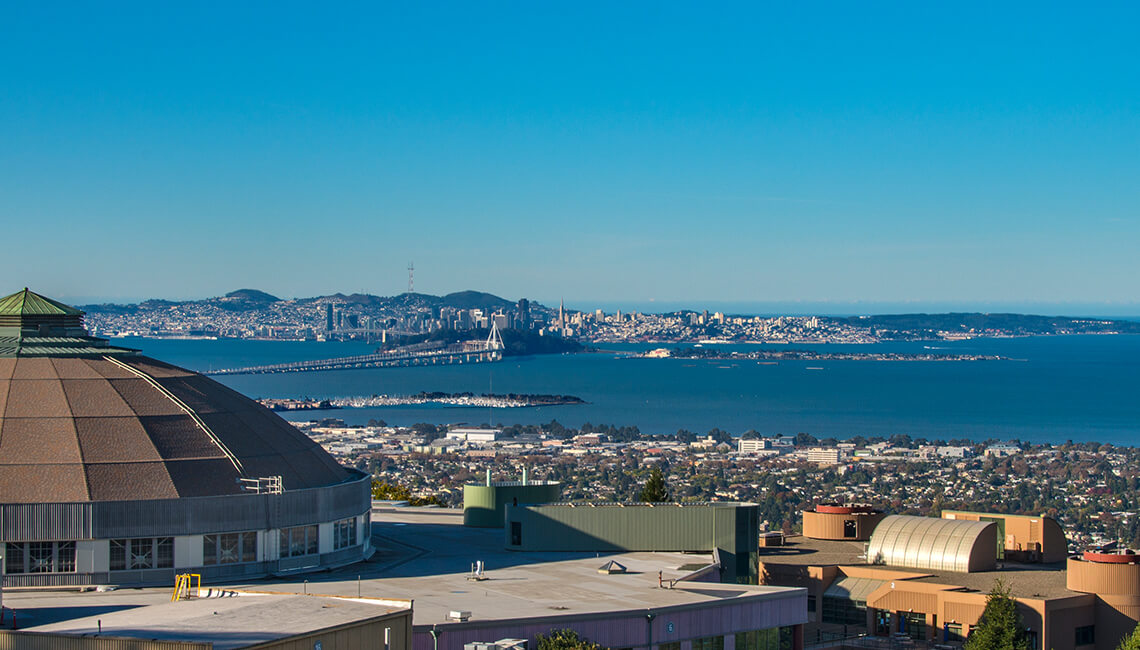
\includegraphics[width=0.8\textwidth]{05-resources/img/spec/lab-view.jpg}
    \caption{Lawrence Berkeley National Laboratory}
    \label{fig:introduction:lbl:view}
\end{figure}


\section{The objectives}
\label{ch:introduction:objectives}

Celeritas is already accelerated by \acrshort{gpu}s, however, the team wants to
improve the performance.
In the current version of the code, each particle track is processed in parallel
by one GPU thread, with no collaboration between threads.
GPU profiling of the code shows that execution time is dominated by two kernels.
The first one is handled by the interaction with the detector geometry to know
where, in 3D space, the particle is situated and during the profiling, the
library used is vecGeom~\cite{VecGeom}.
The second kernel, which will be the focus of this Bachelor thesis project, is
the computation of a differential equation using Dormand-Prince~\cite{princeDormand}.

However, the thesis can be a success even if the project doesn't meet the improvement.
This is because we don't yet know whether thread synchronization will be more
time-consuming than the original version.
In addition, the kernel launch in Celeritas have to be changed, and this
could take up a considerable amount of optimization time.
For the Bachelor thesis, it is sufficient to have a proof of concept that
demonstrates if the enhancement is effective and deserves to be integrated.
To measure the changes done during the internship, the profiler must be run
before and after each step of the project.
The mandatory requirements are described in the following section.

\subsection{Learn GPU programming}
\label{ch:introduction:objectives:learn-gpu-programming}

Before starting to work on the project, some things need to be learned and the goal here is to learn a new way of programming.
To conclude this goal, no code will be produced except for exercises, but the important notions of \acrshort{gpu} programming with CUDA will be synthesized using cheat sheets.
To take advantage of the delay between the beginning of the Bachelor thesis and the beginning of the \acrshort{lbl} internship, this step will be done during this time.


\subsection{Understand the project}
\label{ch:introduction:objectives:understand-the-project}

To be able to improve the performance of the code, the first step is to understand the project and it's always better to understand the background: why it is needed, who will use it and which paradigm and tools are used.

To measure the performance gained, it is necessary to know where the project is at each step.
To take a snapshot of the performance, a profiler can be run and this includes that we can compile and launch the project.
This step will be done at the beginning of the project on-site.


\subsection{Improve the performance}
\label{ch:introduction:objectives:improve-the-performance}

The main goal of the project is to improve the performance of the implementation of Dormand-Prince method~\cite{princeDormand}.
This last mandatory requirement is the core of the thesis and the most important part of the project and it will require the knowledge gained in the first two steps to improve the performance.

To conclude this step, the code must compile, pass the unit test, and a profiler must be run to show the difference between the new and the legacy implementation of the DormandPrince method.
To achieve this goal, the profiles must show an improvement, but this could meet some difficulties to be realized and integrated into the project.
In all cases, the failure of this goal doesn't mean the failure of the thesis if the documentation is correctly done and explains the results obtained and how is it possible or not to continue to this path.
This step will be done after the first two steps and it will take the whole time left.

\section{Optional requirements}
\label{ch:introduction:optional-requirements}

These optional goals are good additions to the project but they are not
require to have a concrete result.

The first one is to have a portable performance.
The purpose of Celeritas is to be run on all kinds of \acrshort{gpu} and even on machines with just a \acrshort{cpu}.
During the optimization, the improvement will be checked on the Perlmutter~\cite{Perlmutter} which uses Nvidia A100 with the architecture Ampere~\cite{ampere} and some improvement can be only effective to this kind of \acrshort{gpu}.
This goal is here to check if the improvement has a positive effect on other architectures and if it is not, to find a way to do that.
To begin this step, the main goal needs to be finished.

The second optional objective is to do another performance improvement.
If the performance of the Runge-Kutta method~\cite{Runge-Kutta-methods} is improved, another optimization can be done.
This part goal will be discussed further in the project with the supervisors and the customers and it will be managed like the last mandatory goal.
This step can be done multiple times if there is enough time.
